\chapter{Asking Salt Lake City Millionaires How They Got Rich}

This chapter is built from an interview lecture rather than a blackboard lecture, but it still has a definite quantitative spine. We move from teaser claims of scale, to execution under a new technological regime, to a real-estate compounding mechanism, to accounting control and arbitrage, and finally to concentration, lifestyle compression, and anti-entitlement. The aim here is to keep the spoken order of the lecture while formalizing only the arithmetic that the speakers themselves motivate.

\section{Opening Stakes}

The lecture opens with a montage of wealth signals rather than an argument. A Cybertruck, a sequence of large annual earnings, many companies, and the claim that one could restart from a modest wage and return to millionaire status in less than a year are placed before us as narrative pressure. We are meant to ask not merely whether these people are rich, but whether the path to wealth is reproducible.

The host then states the governing problem in plain language: we are going through wealthy parts of Salt Lake City to ask business owners how they became wealthy and what a younger entrant can do now. This is important for the structure of the notes. The lecture is not trying to produce one universal formula at the outset; it is assembling cases, and the mathematics emerges only when a speaker gives a mechanism precise enough to formalize.

\section{Execution, Timing, and Recovery}

The first full case begins from scarcity. We are told that the entrepreneur came to Utah with \$50 and later did over \$600 million in roughly a decade. When asked how such a jump was made, the answer is deliberately compressed to a single refrain: execution. That refrain is less a slogan than a framing principle for everything that follows.

The first concrete decision named in the interview is the building of the biggest Bitcoin mining facility in Utah in 2014. The striking part is that the move is described as partly accidental: the firm was already a computer company, already had video cards, and simply connected the hardware and began mining. From there the lecture broadens into a thesis about technological timing. Blockchain, tokenization, and AI are presented as new infrastructure layers, much as the internet was in the early 1990s, when many still thought it was a scam.

In that sense the first entrepreneur offers not a detailed market model, but a timing model: enter early when the underlying rails are still being built. The lecture then sharpens the claim further by pointing to tokenization of real-world assets and mentioning the early involvement of BlackRock. We should read this as an interview claim about future economic structure, not as a settled theorem; still, within the lecture it has a clear function. It tells us that execution matters most when joined to a frontier that the majority has not yet priced correctly.

\subsection{Question \& Answer}

The lecture then raises the first real tension: what happens when the operator does not merely risk money, but loses a huge amount of it very quickly?

The answer is severe. A bad marketing manager loses \$800{,}000 in 90 days. The company has to lay off 75 people. The story matters because it interrupts the easy glamour of the opening montage and forces the lecture to ask what remains after a violent operational error.

The recovery logic is presented as an ordered sequence rather than as a general principle:

\begin{enumerate}
\item stop the immediate damage;
\item cut the cost structure, even brutally;
\item return to the books and rebuild operational visibility;
\item consult strong mentors;
\item frame the problem cleanly;
\item execute again.
\end{enumerate}

The striking claim is that this sequence led to recovery within 12 months. The lecture does not offer a cash-flow table here, and we should not invent one. What it does offer is a recoverability algorithm: execution after failure is not mystical confidence, but disciplined reduction back to controllable variables.

This is why the next question follows so naturally. If everything were lost tomorrow, could it all be made back? The answer is yes, and the compressed reason is selling. That becomes the bridge back to technology. The entrepreneur then says that blockchain and AI now resemble the early internet: a field that looks strange to outsiders, but in which fresh problems will generate fresh fortunes for those who arrive early enough to solve them.

\section{Real Estate as a Compounding Machine}

After a brief recap and transition, the lecture pivots to Chris Krohn and changes its center of gravity. We are no longer primarily in a frontier-tech story. We are now in a capital-recycling story.

The origin story is already stated in quantitative terms. The speaker says he began with a small portfolio of 25 homes, enough that when he graduated college he did not need to get a job, and that this later turned into thousands of homes. He also states that he has made over \$10 million in a single year. The lecture is now asking for mechanism rather than mythology.

\subsection{Question \& Answer}

The natural question is immediate: if there is a common misconception that one needs a great deal of money to start building wealth in real estate, what is the first actionable move?

The answer is house hacking. We can formalize the verbal structure of that answer without pretending that the lecture supplied a full underwriting model.

\begin{definition}
For house \(n\), let \(P_n\) denote the purchase price, \(V_n\) the market value, \(L_n\) the loan balance, \(D_n\) the down payment, and \(E_n\) the equity.
\end{definition}

The lecture gives us the first step directly:
\begin{align}
D_1 &= 0.03 P_1,\\
P_1 &< V_1,\\
E_n &= V_n - L_n.
\end{align}

The verbal logic is then this: the first house is purchased with a \(3\%\) down payment and below market. That creates embedded equity. Some portion of that equity is then stripped out and used to seed the next acquisition. In schematic form,
\begin{equation}
E_1 \rightsquigarrow D_2,\qquad E_2 \rightsquigarrow D_3.
\end{equation}

The lecture is not giving us refinance ratios, time lags, or exact loan terms. What it is giving us is a recursive capital ladder.

\paragraph{Worked chain.}
We can write the logic of the sequence as follows.

\begin{enumerate}
\item Acquire the first house with a small down payment:
\[
D_1 = 0.03 P_1.
\]
\item Buy below market:
\[
P_1 < V_1.
\]
\item The gap between market value and debt creates equity:
\[
E_1 = V_1 - L_1.
\]
\item Extract some usable portion of \(E_1\) and redeploy it as the next down payment \(D_2\).
\item Repeat the same logic at the next step, so that one property helps fund the next.
\end{enumerate}

This is not yet a proof of infinite compounding, and the lecture does not pretend otherwise. It is the more modest claim that capital can be made to move recursively rather than linearly.

\begin{figure}
\centering
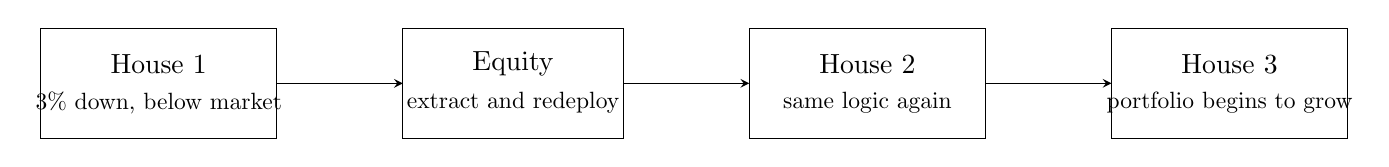
\begin{tikzpicture}[x=1cm,y=1cm,>=stealth]
\draw (0,0) rectangle (3,1.4);
\node at (1.5,0.95) {House 1};
\node[scale=0.85] at (1.5,0.45) {$3\%$ down, below market};

\draw[->] (3,0.7) -- (4.6,0.7);
\draw (4.6,0) rectangle (7.4,1.4);
\node at (6,0.95) {Equity};
\node[scale=0.85] at (6,0.45) {extract and redeploy};

\draw[->] (7.4,0.7) -- (9,0.7);
\draw (9,0) rectangle (12,1.4);
\node at (10.5,0.95) {House 2};
\node[scale=0.85] at (10.5,0.45) {same logic again};

\draw[->] (12,0.7) -- (13.6,0.7);
\draw (13.6,0) rectangle (16.6,1.4);
\node at (15.1,0.95) {House 3};
\node[scale=0.85] at (15.1,0.45) {portfolio begins to grow};
\end{tikzpicture}
\caption{Transcript-derived capital ladder for the house-hacking sequence. The lecture gives the structure verbally: one asset seeds the next through equity extraction.}
\end{figure}

The last point in this real-estate answer is also important. The transcript appears to garble the precise wording, but the intended claim is clear enough: high-volume real-estate activity is not imagined as waiting passively to accumulate a great pile of initial cash. It is imagined as learning how to make capital move.

\section{Reading the Business Like an Owner}

The lecture next makes a decisive shift. Having described how an asset ladder is started, the speaker turns to a common business mistake: owners trust their accountants and their CFOs too much. That criticism is not anti-accounting; on the contrary, it is a demand that the owner learn the accounting language directly.

\begin{definition}
Let \(R\) denote gross revenue, \(X\) expenses, \(\Pi\) retained profit, and \(m\) margin.
\end{definition}

The minimal bookkeeping identities are then
\begin{align}
\Pi &= R - X,\\
m &= \frac{\Pi}{R}.
\end{align}

The lecture's point is operational. One may be very good at creating revenue and still fail to keep much of it. If the owner cannot read the numbers directly, then another party is effectively deciding what the business means. The phrase ``the language of business is accounting'' should be taken seriously. In this interview, accounting is not clerical afterthought; it is the grammar of control.

\subsection{Question \& Answer}

The natural next question is stated explicitly: what lesson about money would someone fail to learn in business school?

The answer is financial arbitrage. The lecture presents it in the simplest possible form. If capital can be borrowed at a low rate and deployed at a much higher rate, the difference is where wealth is made.

We can formalize the verbal structure by writing
\begin{align}
\Delta r &= r_{\text{earn}} - r_{\text{borrow}},\\
W_{\text{spread}} &= K\,\Delta r = K\,(r_{\text{earn}} - r_{\text{borrow}}),
\end{align}
where \(K\) is the deployed capital, \(r_{\text{borrow}}\) is the borrowing rate, and \(r_{\text{earn}}\) is the return earned on the deployment.

The lecture supplies example rates rather than a complete model:
\[
r_{\text{borrow}} \in \{3\%,5\%,7\%\},\qquad
r_{\text{earn}} \in \{25\%,50\%,100\%\}.
\]

\paragraph{Worked example.}
Take the midrange illustrative pair
\[
r_{\text{borrow}} = 5\%,\qquad r_{\text{earn}} = 25\%.
\]
Then
\[
\Delta r = 25\% - 5\% = 20\%,
\]
and so
\[
W_{\text{spread}} = 0.20\,K.
\]

This is exactly the kind of compact arithmetic the lecture likes. The spread is called ``the middle part.'' The speaker's additional claim is that one must be smart enough not to surrender this middle part by giving too much authority over capital to other people. We should also be careful here. The interview does not give taxes, default probabilities, leverage caps, or timing conventions, so the formula remains a heuristic spread model, not a full finance derivation.

\section{Concentration, Lifestyle, and Capital Allocation}

The Keaton Hoskins segment radicalizes the lecture. The first claim is biographical---entrepreneurship as a total identity, many companies built since the age of 21, more than \$10 million earned---but the real center is a doctrine of allocation.

The doctrine begins with lifestyle compression. One should learn how to downgrade one's lifestyle so that one can later upgrade one's life. This is immediately tied to a quoted numerical claim: one in four millionaires still live paycheck to paycheck because they refuse to compress lifestyle, even temporarily. The lecture does not prove that statistic; it uses it to sharpen the difference between wealth and consumption.

The next step is a two-channel rule for capital deployment. In the speaker's formulation, money should be dumped into only two things: the self and the company. The more money he puts into himself, the more he makes; the more money he puts into the business, the more the business makes. The important move here is not abstract frugality. It is concentration of reinvestment into the few channels thought to have compounding power.

That concentration thesis becomes explicit when diversification is attacked. The lecture does this rhetorically, but the arithmetic beneath the rhetoric is clear enough to write down. Let \(a_i\) denote the fraction of total available effort, capital, or attention placed into project \(i\). Then
\begin{equation}
\sum_{i=1}^{N} a_i = 1.
\end{equation}

If one spreads oneself over five directions at once, the lecture's model is
\begin{equation}
a_i = 0.2\qquad (i=1,\dots,5).
\end{equation}
If one goes all in on a single direction, it becomes
\begin{equation}
a_1 = 1.
\end{equation}

The speaker's claim is that the second pattern, not the first, reaches anything of significance. In his phrasing, one should forget the portfolio fantasy and go deep.

\begin{remark}
This is not a theorem of optimal portfolio construction. It is a motivational concentration model: significance is said to require depth before breadth.
\end{remark}

The lecture then gives a vivid version of the same point. Someone arrives with \$100{,}000 and wants to do stocks, Bitcoin, start a business, buy a business, and several other things at once. The speaker's answer is no: find one thing you can get behind. Here again the chapter's task is not to intensify the rhetoric, but to preserve the mechanism. Splitting scarce attention widely is treated as a way of guaranteeing mediocrity.

\section{Not Being Broke: Cash Management and Entitlement}

The final movement returns from allocation to a more primitive question: what does it mean to be broke? The answer is unexpectedly strict. The speaker says he has never really been broke, even though he had only \$100 in his bank account at age 21 and again when his father died. The reason is that he does not define ``broke'' merely as low balance. He defines it as dependence, as being in a place where somebody else must rescue him.

That leads to the most compact heuristic in the lecture:
\begin{equation}
\neg \mathrm{Manage}(100)\Rightarrow \neg \mathrm{Manage}(10^5),\qquad
\neg \mathrm{Manage}(100)\Rightarrow \neg \mathrm{Manage}(10^6).
\end{equation}
This should not be mistaken for a law of economics. It is a behavioral scaling rule. If one cannot manage \$100, then more money will not cure the problem; it will merely magnify it.

From there the lecture gives a stylized austerity program. If income fell to \$3{,}000 per month, the speaker says he would share housing, minimize transport, cook meals, repeat clothing, and cut spending on anything not strictly needed. The transcript does not specify an exact per-person rent because the number of roommates is not fully pinned down, but the structure is clear: fixed lifestyle costs must collapse before capital can accumulate.

The deeper diagnosis is then named directly. What keeps people broke is not only low income, but entitlement. People spend too much money on things they do not need, and they assume they are owed a certain house, a certain car, a certain visible level of consumption. The lecture is emphatic that no one is coming to save them. Again, we should preserve the mechanism beneath the rhetoric. Entitlement produces rigid expenses; rigid expenses destroy investable surplus.

A good way to summarize the final doctrine is this:

\begin{itemize}
\item low balances are survivable;
\item unmanaged spending is not;
\item status consumption competes directly with capital formation;
\item temporary austerity is presented as the price of independence.
\end{itemize}

The interview closes by widening the point into cultural language. Hard workers with low entitlement are contrasted with those who assume they deserve a fully formed lifestyle before they have earned it. Whether or not one agrees with every example, the lecture's mechanism is unmistakable: overspending and entitlement are treated as mathematical enemies of compounding.

\section{Summary}

This lecture begins by dazzling us with visible wealth and then spends the rest of its time explaining why the visible layer is not the real one. The deeper layer is execution under a new technological regime, recovery after catastrophic loss, recursive capital movement in real estate, owner-level accounting control, spread capture through arbitrage, concentration of effort, and refusal of entitlement. The chapter's mathematics is therefore modest but definite: equity is recycled, margins are read, spreads are computed, attention is allocated, and small-scale cash management predicts large-scale outcomes. That is the commercial arithmetic by which the lecture says wealth is built.